\subsection{Performance Considerations}
\label{sec:performance}

The performance of the different propagation algorithms, quantified by
the time it takes to simulate a certain number of propagation steps, is
about the same. The number of propagation steps, however, which is
determined by the number of scatterings, has a significant effect on the
total simulation time.

Figure \ref{fig:Go7Maquo} shows a comparison of the
standard-\clsim algorithm (section \ref{sec:standard_clsim}), the
hole-ice-correction algorithm (section \ref{sec:algorithm_a}), and the
new medium-propagation algorithm with hole ice (section
\ref{sec:algorithm_b}), each running a simulation propagating \(10^5\)
photons on a
CPU.\footnote{Test system configuration for CPU simulation: OS: macOS Sierra 10.12.6 16G1212 x86\_64, Kernel: 16.7.0, CPU: Intel i7-4870HQ (8) @ 2.50GHz, GPU: Intel Iris Pro, NVIDIA GeForce GT 750M, RAM: 16384MiB.}

\begin{figure}[htbp]
  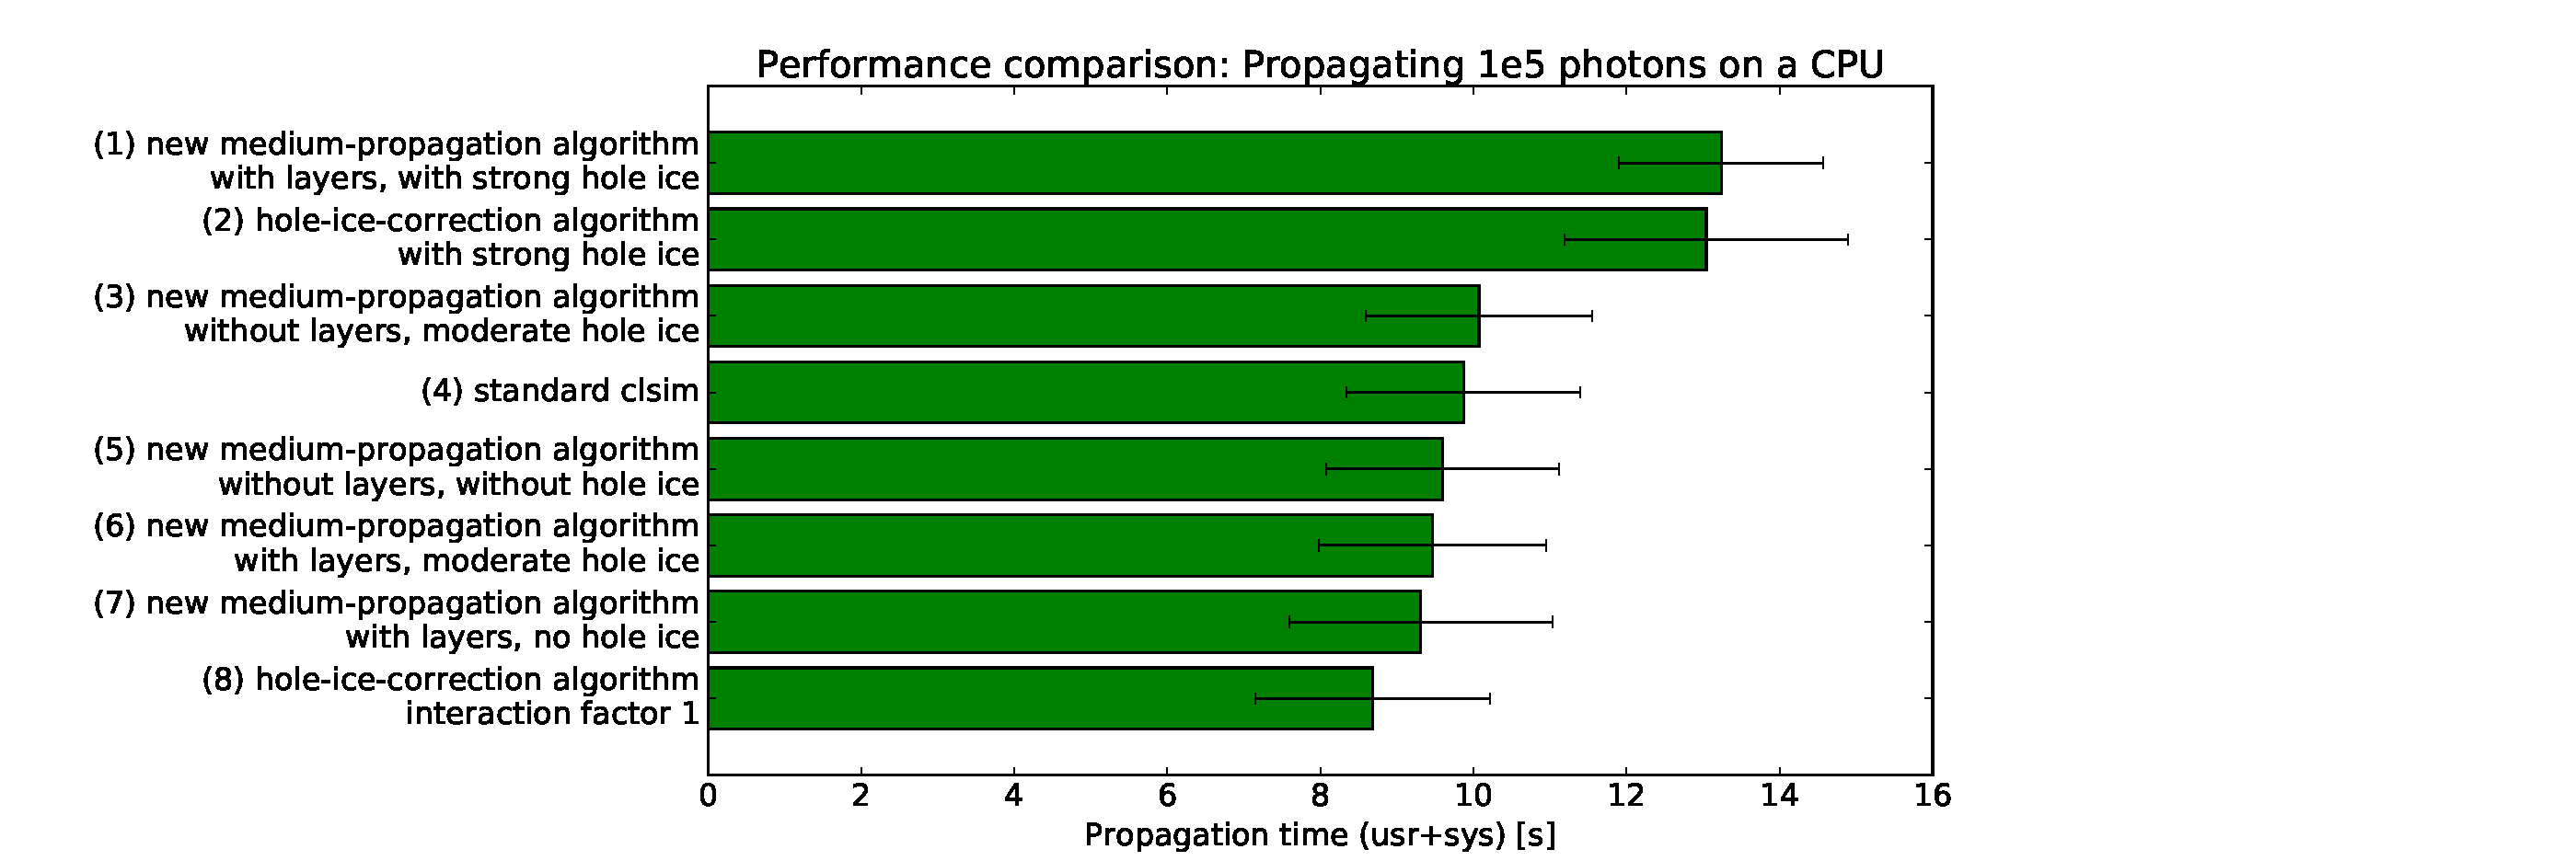
\includegraphics[width=\textwidth, trim = {1cm 0 10cm 0.7cm}, clip]{img/performance-comparison}
  \caption{Performance comparison different hole-ice algorithms and different hole-ice scenarios.}
  \label{fig:Go7Maquo}
\end{figure}

\docpar{The implementation of this performance measurement is documented in \issue{49}.}

The difference of the total simulation time for each algorithm is
smaller than the statistical uncertainty of the time measurement as long
as the scattering length of the hole-ice cylinder is kept moderate (rows
3 to 8 in figure \ref{fig:Go7Maquo}). When moving to smaller scattering
lengths within the hole-ice, however, the total simulation time
increases (rows 1 and 2 in figure \ref{fig:Go7Maquo}), as the total
number of simulation steps increases, because one simulation step
propagates the photon from one scattering point to the next scattering
point. For a fixed hole-ice-cylinder radius of \(30\cm\), going from a
geometric hole-ice scattering length of \(20\m\) to \(0.005\m\)
increases CPU propagation time per photon by about \(15\,\%\).

The same effect can be observed when comparing the run time of flasher
simulations on a
GPU.\footnote{Test system configuration for GPU simulation: Scientific Linux release 7.4 (Nitrogen) x86\_64, Kernel: 3.10.0-862.6.3.el7.x86\_64, CPU: Intel Xeon E5-2660 0 (32) @ 3.000GHz, GPU: NVIDIA Tesla K20m, RAM: 64215 MiB}
Running a flasher simulation with standard \clsim using hole-ice
approximation takes about 11 minutes. Running the same simulation with
the same number of photons, with the new medium-propagation algorithm,
but without any hole-ice cylinders takes about 10 minutes. Running the
same simulation, but adding hole-ice cylinders with \(36\cm\) radius and
a scattering length of \(\sfrac{1}{10}\) of the surrounding bulk ice
takes about 15 minutes, increasing the simulation time by about
\(50\,\%\).

As the number of simulation steps is the dominant factor for the
required simulation time, it is desirable to further optimize the
implementation of the simulation step (section
\ref{sec:technical_issues_and_optimizations}), because even small
improvements, multiplied by the number increased number of scattering
steps for hole-ice simulations, cause a considerable total performance
gain.\followup

These performance considerations also lead to the question when it is
most useful to use hole-ice propagation algorithms and when to use the
default hole-ice approximation with effective angular-sensitivity
curves. The approximation does not consider the effective reflection of
photons when entering the hole ice (section
\ref{sec:scattering_simulation}), but only removes a certain percentage
of photons for each incoming angle. Also, the approximation considers
each optical module perfectly centered within the hole ice rather than
accounting for the individual displacement of each module. In
high-energy events with large statistics where many photons and many
different optical modules are involved, the displacement effects are
expected to cancel out and the reflection effects are expected to be
negligible. For these scenarios, in particular for events with long
high-energy muon tracks, the hole-ice approximation is expected to be
sufficient. For lower-energy events and events where only a few optical
modules are involved, using a calibrated direct photon propagation
simulation is expected to reduce simulation systematics. Further
studies, however, are required to quantify this reduction of
systematics, or equivalently to quantify the gain in precision.\followup
